\section{Key Characteristics}
\begin{figure}[t]
\centering
    \subfigure[\label{subfig:end_to_end_training}End-to-End Model Training and Deployment]{
    \centering
    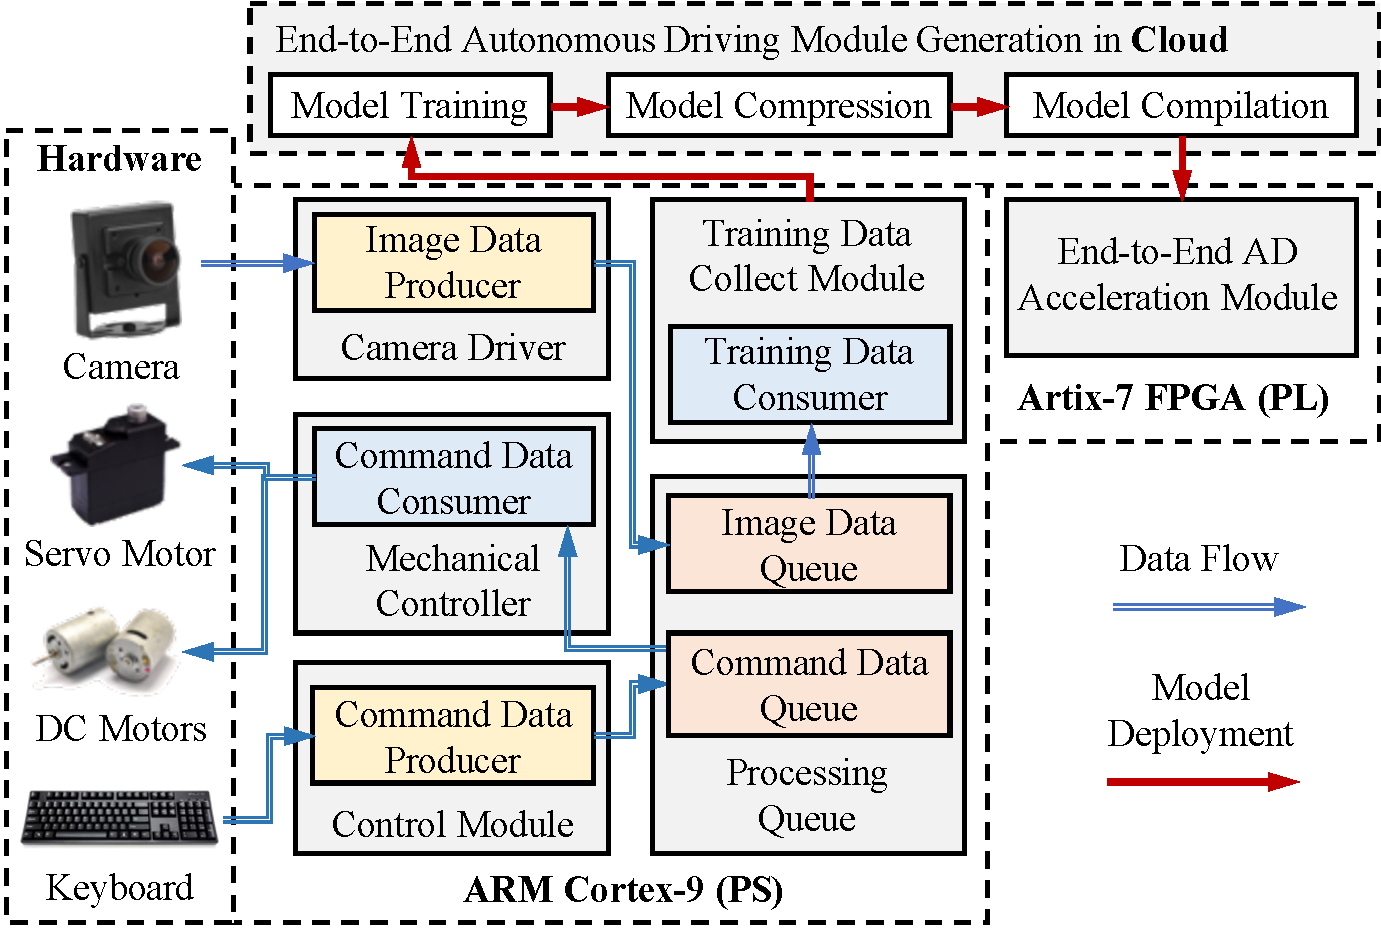
\includegraphics[width=3.4in]{end_to_end_training}
    }
    \vspace{0.1in}
    \subfigure[\label{subfig:end_to_end_inference}End-to-End Model Inference Data Flow]{
    \centering
    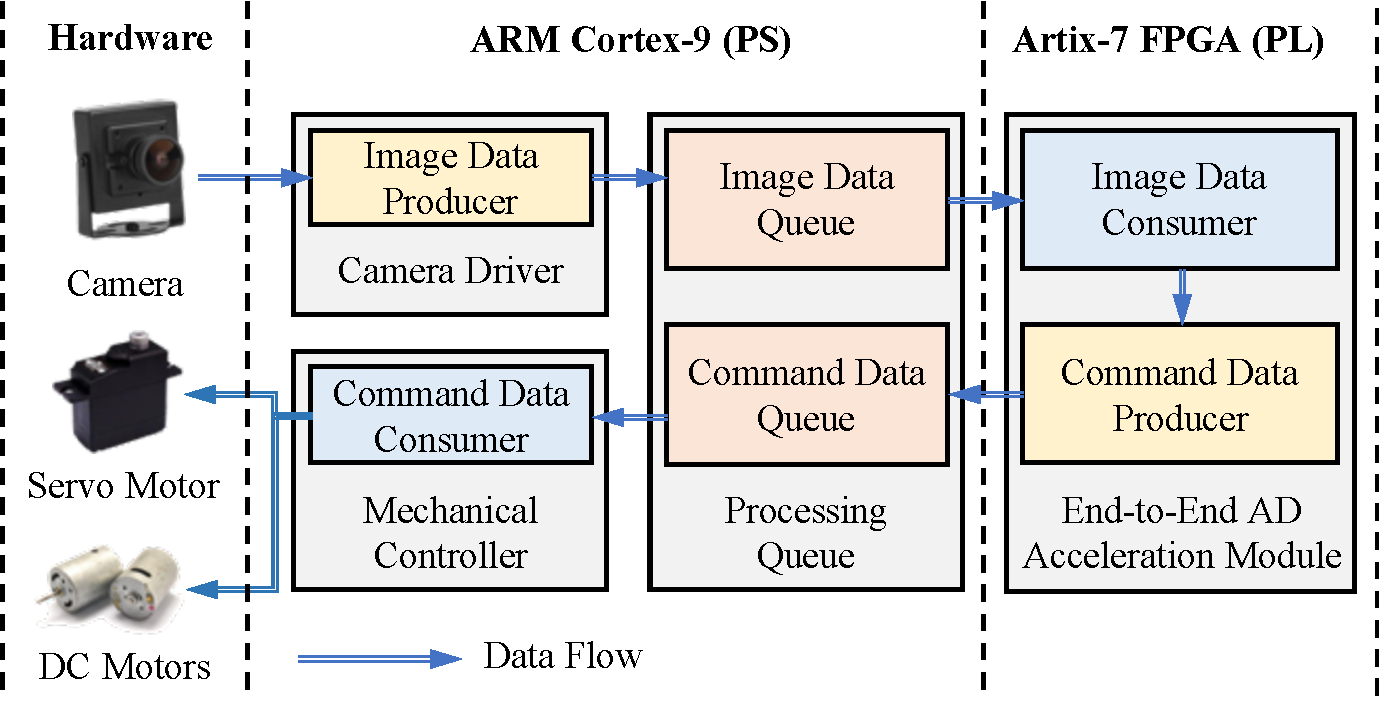
\includegraphics[width=3.4in]{end_to_end_inference}
    }
\caption{Autonomous Driving using End-to-End Model.}
\label{fig:end_to_end_autonomous_driving}
\end{figure}
The HydraMini platform has three key characteristics: high flexibility and extensibility, full stack, and easy-to-use. These three characteristics help users understand AD technology stack and the platform.

\textbf{High Flexibility and Extensibility. }The idea of our system design is inspired by ROS. In ROS, new functions are easily added by adding ROS nodes. Nodes get and send messages easily through the publish-subscribe mechanism. What we do is making the ROS system more lightweight and forthright. The thread is similar to node while the producer–consumer model is similar to the publish-subscribe mechanism. So it's easy to add more hardware devices as sensors or threads as handlers. What's more, due to the base of our system is Ubuntu18.04, it's easy to redefine the whole software framework as you like, actually we have an example of using ROS in following case studies.

\textbf{Full Stack. }The full stack here means our product provide almost everything you need to learn about AD technologies from algorithms to hardware. It's important for researchers or students to understand how the car runs and why sophisticated algorithms are able to run in resource limited edge platform. Users could use different physical construction, different operating system, different software framework, different algorithm and different hardware acceleration etc. That means researchers are able to do whatever research they want based on our platform and they could use existing modules and understand the operation mode of the whole system. Considering the difficulty users may have in collecting training data and testing AI models in real world, we provide a simulator modified from sdsandbox\cite{sdsandbox} which is first used in Donkey Car\cite{donkeycar}. The simulator is used to do tests or more. Its usage will be introduced in case studies.

\textbf{Easy-to-Use. }The most important thing we believe is to make our platform easy to use. To achieve this, most libraries of the platform are familiar to users like OpenCV and TensorFlow\cite{tensorflow}, they are open-sourced and widely used. Most importantly, the basic knowledge users should know includes only Linux, C++, Python, AI and a little about DPU usage. The software framework is simple and tidy, we only keep necessary functions and make it extendable. The hardware is simple too, if you don't want to add more devices, one camera and two motors are all you have to deal with. Users even don't have to prepare a real car to do experiments, then you care nothing about hardware. Besides, we provide many documents for users, so it's easy for them to modify any part of the platform.